\documentclass[11pt, a4, nocenter, margin=150mm]{article}

\usepackage[top=20mm, bottom=20mm, inner=25mm, outer=25mm]{geometry}
\usepackage[title, toc]{appendix}
\usepackage{array}
\usepackage[font=scriptsize, labelfont=it, textfont=it]{caption}
\usepackage{graphicx}
\usepackage{setspace}
\usepackage{enumitem}
\usepackage[parfill]{parskip}
\usepackage{nameref}
\usepackage{multirow}

\setlength{\parindent}{0pt}

\begin{document}

%%%%%%%%%%%%%%%%%%%%%%%%%%%%%%%%%%%%%%%%%%%%%%%%%%%%%%%%%%%%%%%%%%%%%%%%%%%%%%%%
\onehalfspacing
\begin{titlepage}
	\begin{center}
		\Huge
		\textbf{UNSW} \\

		\vspace{5mm}

		
\includegraphics[height=4cm]{unsw-logo.jpg}

		\vspace{5mm}

		\Large
		Faculty of Engineering \\
		School of Computer Science \& Engineering \\

		\vspace{10mm}

		\textbf{COMP3431} \\
		Robot Software Architectures \\

		\vspace{15mm}

		\LARGE
		\textbf{Project 1 Individual Report} \\
		
		\Large
		Group: Bob Ros

		\vspace{15mm}

		\Large
		Course Coordinator: Claude Sammut\\
		Due Date: 16/09/2020 \\

		\vfill
		\rule{\linewidth}{0.5pt} \\

		\Large
		Dan Nguyen \\

		\large
		z5206032 \\

	\end{center}
\end{titlepage}

%%%%%%%%%%%%%%%%%%%%%%%%%%%%%%%%%%%%%%%%%%%%%%%%%%%%%%%%%%%%%%%%%%%%%%%%%%%%%%%%
\pagenumbering{roman}
\tableofcontents
\vspace{1cm}
\listoffigures
\vspace{1cm}
\pagebreak

\pagenumbering{arabic}

%%%%%%%%%%%%%%%%%%%%%%%%%%%%%%%%%%%%%%%%%%%%%%%%%%%%%%%%%%%%%%%%%%%%%%%%%%%%%%%%
\section{Tasks}
\label{sec:tasks}
	The project tasks are summarised and divided like so (following the recommendation of the assignment specifications):

	\begin{enumerate}[noitemsep, nolistsep]
		\item Mapping: Explore world, building a map and keep tracking of the trajectory.
		\item Exploration: Autonomously navigate world frontiers.
		\item Waypoint Navigation: Return to home once all AR markers are located.
		\item Vision Processing: Locate and place AR markers on the map.
	\end{enumerate}

	In order to solve these tasks, ROS packages are to be researched, selected and integrated into the final solution. This is discussed in the next section under relevant task subsections.

\section{ROS Packages}
\label{sec:packages}

	\subsection{Mapping}
	\label{sec:mapping}

		Packages explored were:
		\begin{itemize}[noitemsep, nolistsep]
			\item GMapping
			\item Hector Slam
			\item Cartographer
		\end{itemize}

		For the course-provided maze world, package were compared to determine the most appropriate SLAM technique. Each SLAM package was simple to install using APT and easy to run (instructions in Appendix \ref{app:slam_instructions}). A trend existed in increasing map quality with recency of the 2D SLAM technique.
		
		GMapping (Figure \ref{fig:gmap_result} below) was released in 2010 and generates the worst map due to its reliance on wheel odometry for localisation. This causes sections of the map to appear to have "drifted" when stitched to the global map, therefore reducing the map accuracy. No further research went into GMapping for its trajectory information as its map result was unsatisfactory.

		\begin{figure}[h!]
			\centering
			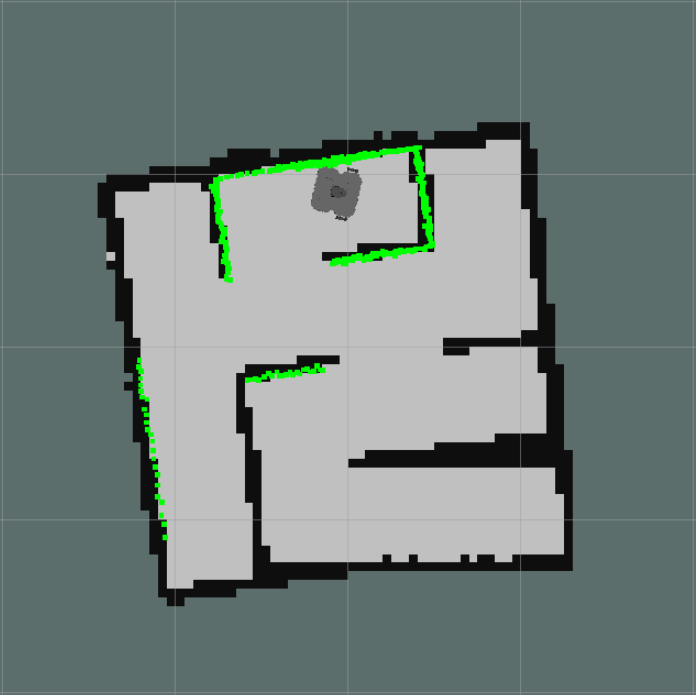
\includegraphics[width=50mm]{../slam/gmapping_1.png}
			\caption{GMapping Map}
			\label{fig:gmap_result}
		\end{figure}


		Hector slam (Figure \ref{fig:hector_result} below) was released in 2012 and generates a good map. This slam technique uses iterative closest point odometry with laser scan data producing more accurate map results. Trajectory required installation of the hector\_geotiff package and launching a geotiff\_mapper.launch node.

		\begin{figure}[h!]
			\centering
			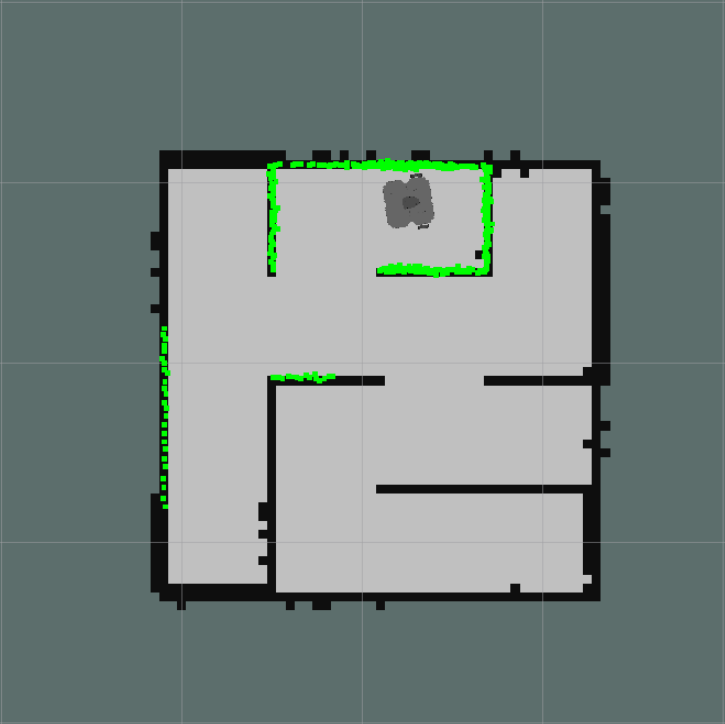
\includegraphics[width=50mm]{../slam/hector_1.png}
			\caption{Hector Slam Map}
			\label{fig:hector_result}
		\end{figure}

		Cartographer (Figure \ref{fig:cartographer_result} below) was released in 2018 and generates the best quality map. Trajectory is included in the cartographer-ros package and is a display option in RVIZ and requires no additional installation or nodes.

		\begin{figure}[h!]
			\centering
			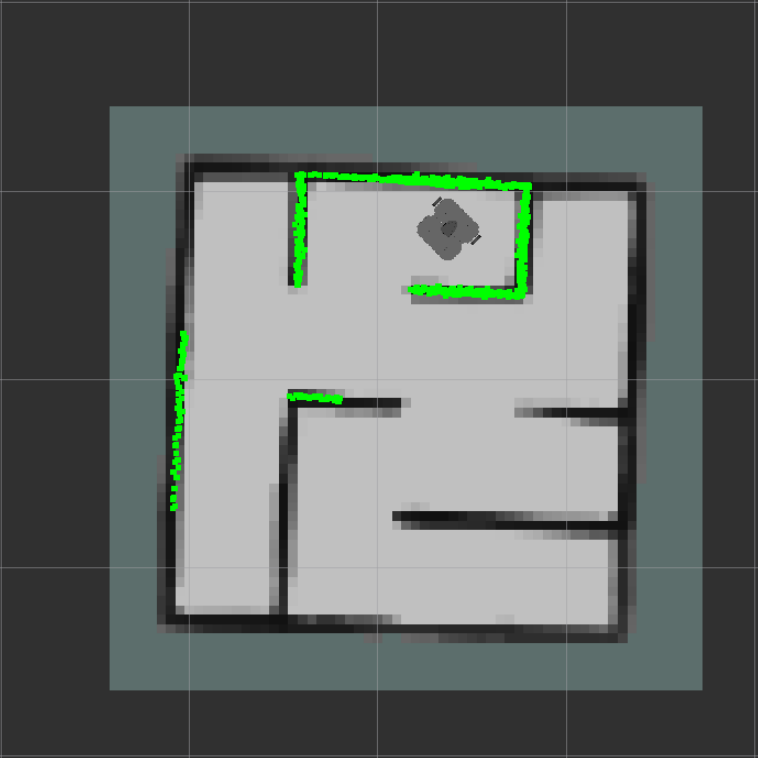
\includegraphics[width=50mm]{../slam/cartographer_1.png}
			\caption{Cartographer Map}
			\label{fig:cartographer_result}
		\end{figure}

		Ultimately, cartographer was selected due to its more accurate map result and default display trajectory option in RVIZ to solve the task of mapping. Ease of installation was negligible.

	\subsection{Exploration}
	\label{sec:explore}

	Packages explored were:
	\begin{itemize}[noitemsep, nolistsep]
		\item Frontier Exploration
		\item Explore-lite
	\end{itemize}

	From online rumours, frontier exploration was no longer supported for the Melodic distribution (this is confirmed by no available APT package). However, the frontier exploration project on GitHub had a melodic-devel branch which prompted personal interest in building the package. Building and running frontier exploration showed problems related to its server-client feature i.e. frontier exploration was not communicating with any active topics (see Figure \ref{fig:frontier_error}).

	\begin{figure}[h!]
		\centering
		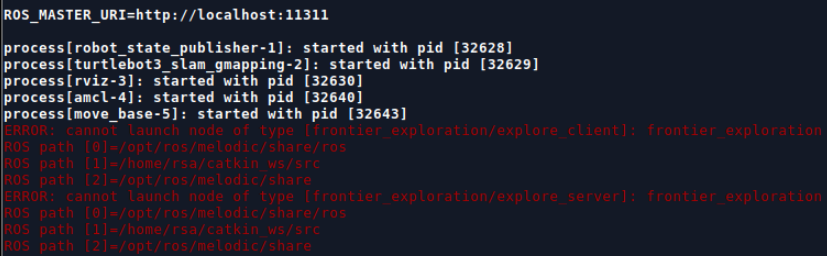
\includegraphics[width=120mm]{frontier-error.png}
		\caption{Frontier Exploration Error}
		\label{fig:frontier_error}
	\end{figure}

	Explore-lite is a derivative of frontier exploration designed as a light-weight SLAM. Running explore-lite revealed problems with the course-provided maze.launch world where the simulated turtlebot3 had difficulty in searching for a starting position (see Figure \ref{fig:explore_lite_warning}). This problem did not exist for large worlds, therefore it can be deduced that the turtlebot3 and wall boundaries were overlapped. As explore-lite did not show promise in simulation, we decided to use wallFollower.cpp to explore the map as the more reliable and quick-to-implement solution.

	\begin{figure}[h!]
		\centering
		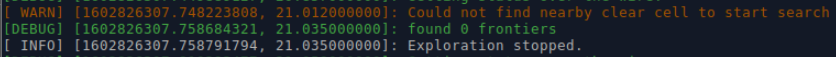
\includegraphics[width=120mm]{explore-lite-warning.png}
		\caption{Explore-lite Warning}
		\label{fig:explore_lite_warning}
	\end{figure}
	
	The provided wall following algorithm had a major problem of alternating between states at intersections (which causes the turtlebot3 to appear to have stopped or pendulate). This prompted research into existing wall following algorithms and attempts to improve the given algorithm (see Appendix \ref{app:wall_follower_algorithm}). A good wall following algorithm would have more subdivisions of its point clouds and many switch cases to select a heading, which was considered too verbose for this project. Therefore, the original wall follower code was used which had satisfactory performance to autonomously navigate the world.

	\subsection{Waypoint Navigation}
	\label{sec:navigation}

	No ROS packages were explored for navigation as wall following was decided as the exploration method. To navigate home, a listener was written in wallFollower.cpp to stop at home if the turtlebot3 was within the home boundary (see Appendix \ref{app:homing_algorithm}). The initial implementation involved writing a submap listener which was published by cartographer. This worked well in simulation but caused conflicts in the transform tree on the turtlebot3 in the lab. The adhoc solution was to rewrite the listener to listen to the odometry topic. This was highly unreliable as pose.position had large positional drift exacerbated by turtlebot3 turns.

	\subsection{Vision Processing}
	\label{sec:vision}

	Packages explored were:
	\begin{itemize}[noitemsep, nolistsep]
		\item Aruco \& OpenCV
		\item AR Track Alvar \& ROS
	\end{itemize}

	Aruco and OpenCV was considered for its more powerful functionality for manually mapping laser scans with AR marker positioning therefore leading to more accurate localisation. This option worked but was difficult to integrate with the existing solution as well as its incompatibility with the marker dictionaries.

	The package solution for the vision processing task was AR tracker alvar which has built in dictionaries to interface with the AR markers and was easily integrable into the existing solution. The AR marker solutions are mapped onto RVIZ as shown in Figure \ref{fig:ar_markers}.

	\begin{figure}[h!]
		\centering
		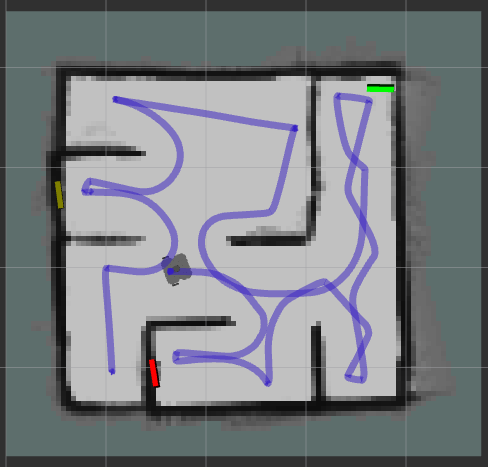
\includegraphics[width=120mm]{ar-markers.png}
		\caption{AR Mapping}
		\label{fig:ar_markers}
	\end{figure}

\section{Evaluation \& Limitations}
\label{sec:evaluate}

	Bob Ros scored 9/10. The turtlebot3's performance was very good in traversing the map without collision, and spotting and marking all AR markers on the map.

	0.5 marks was lost for a placement error in AR marker 4. The cause for this was due to the approach of the turtlebot3 to the marker at an extreme angle which caused the marker's misplacement. The marker placement error was minimised by reducing the distance the turtlebot3 was allowed to approach the marker.

	Another 0.5 marks was lost due to the turtlebot3 failing to stop at home as it waited for the odometry position to fall within the home boundary. This was due to odometry's huge positional drift which may cause the odometry positional origin (home boundary) to drift outside the map boundaries. It should be noted that this drift was exacerbated with every turn.

	Limitations on the current robotic software architecture are:
	\begin{itemize}[noitemsep, nolistsep]
		\item Very large turn radius which may cause the turtlebot3 to run into walls or get lost.
		\item Distance and angle between turtlebot3 and marker which can cause marker misplacement.
		\item Left wall following exploration which inherently has an inability to explore certain map structures and possibility of missing AR markers on walls that are never faced by the turtlebot3.
	\end{itemize}

\section{Contribution}
\label{sec:contribution}

	From the work outlined above in section \ref{sec:packages}: \nameref{sec:packages}, my contribution covered mapping, exploration, and waypoint navigation:
	\begin{itemize}[noitemsep, nolistsep]
		\item Researched SLAM packages, identified installation instructions, and selecting an appropriate SLAM.
		\item Investigate exploration packages, and proposing wallFollower.cpp as an alternative solution.
		\item Attempt to rewrite wallFollower.cpp algorithms, refined launch file parameters.
		\item Attempt to implement a "stop at home" feature in wallFollower.cpp.
	\end{itemize}

\pagebreak

\begin{appendices}

\section{SLAM Instructions}
\label{app:slam_instructions}

	The following instructions to install and run SLAM packages assumes ROS Melodic distribution.
	~\\

	\underline{GMapping}
	\begin{verbatim}
		> roslaunch turtlebot3_slam turtlebot3_slam.launch slam_methods:=gmapping
	\end{verbatim}
	~\\

	\underline{Hector Slam}
	\begin{verbatim}
		> sudo apt-get install ros-melodic-hector-slam
		> roslaunch turtlebot3_slam turtlebot3_slam.launch slam_methods:=hector
	\end{verbatim}
	~\\

	\underline{Cartographer:}
	\begin{verbatim}
		> sudo apt-get install ros-melodic-cartographer ros-melodic-cartographer-ros
		  ros-melodic-cartographer-ros-msgs ros-melodic-cartographer-rviz
		> roslaunch turtlebot3_slam turtlebot3_slam.launch slam_methods:=cartographer
	\end{verbatim}

	Running cartographer in the simulation requires editing the following file:
	\begin{verbatim}
		~/catkin_ws/src/turtlebot3/turtlebot3_slam/config/turtlebot3_lds_2d.lua
	\end{verbatim}

	and changing
	\begin{verbatim}
		tracking_frame = "imu_link",
	\end{verbatim}

	to
	\begin{verbatim}
		tracking_frame = "base_footprint",
	\end{verbatim}

\section{Exploration Instructions}
\label{app:explore_instructions}

	The following instructions to install and run exploration packages assumes ROS Melodic distribution.
	~\\

	\underline{Frontier Exploration}
	\begin{verbatim}
		> cd ~/catkin_ws/src
		> git clone https://github.com/paulbovbel/frontier_exploration.git
		> cd ~/catkin_ws
		> catkin_make
		> source ~/devel/setup.bash
		> roslaunch turtlebot3_slam turtlebot3_frontier_exploration.launch
	\end{verbatim}
	~\\

	\underline{Explore-Lite}
	\begin{verbatim}
		> cd ~/catkin_ws/src
		> git clone https://github.com/hrnr/m-explore.git
		> cd ~/catkin_ws
		> catkin_make
		> source ~/devel/setup.bash
		> roslaunch explore_lite explore.launch
	\end{verbatim}

\section{Wall Follower Algorithm}
\label{app:wall_follower_algorithm}

	Pseudo-code of an attempted wall follower algorithm.
	~\\

	\begin{verbatim}
		Get the closest point on our right
		Get the closest point on our left
		Get the closest point in front

		If left is free
		    turn left
		else if left is occupied
		    turn right
		else if left and straight and right are occupied
		    turn 180
		else
		    go straight 
	\end{verbatim}

\section{Homing Algorithm}
\label{app:homing_algorithm}
	
		Pseudo-code for the turtlebot3 to stop at home when at home.
		~\\
	
		\begin{verbatim}
			If time elapsed is greater than 1 minute
			    If current x position is within home x range
			    And if current y position is within home y range
			        Publish 0 velocity
		\end{verbatim}
	

\end{appendices}

\end{document}